\documentclass[
journal=mamobx,
manuscript=article,
%layout=twocolumn
]{achemso}

%\setkeys{acs}{
%	abbreviations = false,
%	articletitle  = false,
%	keywords      = false,
%	maxauthors    = 10,
%	super         = true
%}

% ===== Comment below before submitting:
%\let\titlefont\undefined
%\usepackage[fontsize=11pt]{scrextend}
%\flushbottom
% ===== Up to this point
%
\usepackage[hyperindex,breaklinks,hidelinks,colorlinks,citecolor=blue]{hyperref}
\usepackage{amsmath, amsthm, amssymb, mathtools}    
\usepackage{float}
\DeclareMathOperator*{\argmax}{arg\,max}
%
\usepackage{tabularx}
\usepackage{multirow}
\newcolumntype{C}[1]{>{\centering\let\newline\\\arraybackslash\hspace{0pt}}m{#1}}
%
\usepackage{graphicx}
\DeclareGraphicsExtensions{.pdf,.png}
\graphicspath{{Figures/}}
%\usepackage[outdir=Figures/]{epstopdf}
%
\usepackage{natmove}
%
\usepackage[inline]{enumitem}
%
\usepackage[version=4]{mhchem}
%
\newcommand{\mt}[1]{\boldsymbol{\mathbf{#1}}}          % matrix symbol
\newcommand{\vt}[1]{\boldsymbol{\mathbf{#1}}}          % vector symbol
\newcommand{\angstrom}{\mathring{A}}                   % Angstrom symbol
%
\usepackage{colortbl}
\usepackage{rotating}
\newcommand{\biphasic}[0]{\cellcolor{blue^^2120}{biphasic}}
\newcommand{\lamellae}[0]{\cellcolor{cyan^^2120}{lamellae}}
\newcommand{\defectivelamellae}[0]{\cellcolor{green^^2120}{defective lamellae}}
\newcommand{\saturatedflatinterface}[0]{\cellcolor{yellow^^2125}{saturated flat interface}}
\newcommand{\mesophasic}[0]{\cellcolor{orange^^2120}{mesophasic}}
\newcommand{\curvedinterface}[0]{\cellcolor{red^^2130}{curved interface}}
%
% Packages used only in the revision stage (should be commented out after that)
\usepackage{todonotes}
\usepackage{soulutf8}
\soulregister\cite7
\soulregister\ref7
\soulregister\ce7
\usepackage[utf8]{inputenc}
%

\author{Tiago Lemos}
\email{tlemos@peq.coppe.ufrj.br}
\affiliation{Programa de Engenharia Química da COPPE, Universidade Federal do Rio de Janeiro, Rio de Janeiro, 68542, Brazil}

\author{Charlles Abreu}
\email{abreu@eq.ufrj.br}
\affiliation{Escola de Qu\'imica, Universidade Federal do Rio de Janeiro, Rio de Janeiro, 68542, Brazil}

\author{Jos\'e Carlos Pinto}
\email{pinto@peq.coppe.ufrj.br}
\affiliation{Programa de Engenharia Química da COPPE, Universidade Federal do Rio de Janeiro, Rio de Janeiro, 68542, Brazil}

\title{DPD Simulations of Homopolymer-Copolymer-Homopolymer Mixtures: Effects of Copolymer Structure and Concentration}

\keywords{dissipative particle dynamics; self-assembly; polymer blends; structure factor}

\date{\today}

\begin{document}

\begin{abstract}
Blends prepared by mixing incompatible homopolymers with a compatibilizing copolymer (produced by repeting units that are compatible with each homopolymer) attract high technological interest due to their self-assembling behavior.
In the present work, 281 dissipative particle dynamics (DPD) simulations were performed in order to evaluate the influence of the microstructure and the concentration of the copolymer on properties of these systems.
The results show that alternate copolymers are arranged between the homopolymeric phases while nanodomains rich in each of the components are formed in the copolymeric matrix.
Dispersion in block lengths increases the size of these nanodomains, so that they can properly allocate homopolymer chains.
Besides, dispersions in chain lengths and chemical compositions of diblock copolymers, which can form self-assembled mesostructures, also lead to development of larger mesophase domains.
Larger dispersions of chain lengths and chemical compositions cause the increase of the amount of copolymers necessary to bring about changes in the mixing behavior, when compared to non-dispersed copolymers.
It can be concluded that microstructural properties of the copolymer exert a decisive impact on molecular interactions and, consequently, on the characteristics of the mesophases generated during the blending process.
Therefore, microstructure control methods, stemming from both polymer-reaction engineering and polymer-purification techniques, are important for the design and resulting performance of the analyzed blends.
\end{abstract}

\maketitle

\section{Introduction}
\label{sec:introduction}

In the polymer industry, polymer blends are manufactured to form new materials that combine properties of different polymers without performing polymerization reactions \cite{Baker_2001}.
Blends are also used to produce high-performance materials through simple mixing of cheaper resins, thus making the production more attractive in both technical and commercial terms \cite{Wang_2012}.

However, due to physicochemical incompatibility between polymers, mixing is often ineffective.
To overcome this problem, compatibilizers can be used.
When compatibilizers are added to a blend of immiscible polymers, they promote interfacial adhesion, thus stabilizing the blends and enabling the achievement of desired properties and performance \cite{Baker_2001}.

Frequently, compatibilizers are copolymers that contain segments of the incompatible homopolymers \cite{Baker_2001, Wang_2012, Chuai_2003, Lyatskaya_1996, Yuan_2006}. In this case, the effect of the copolymer structure on the compatibilization process is well established in the cases of linear \cite{Chuai_2003} and graft \cite{Lyatskaya_1996, Wang_2012} copolymers.
In the linear case, tapered copolymers exert higher compatibilizing effect than diblock copolymers, which in turn are more efficient than triblock materials \cite{Yuan_2006, Kim_2006, Lemos_2015}.
It is also known that compatibilizer copolymers with low molecular-weight perform better than their high molecular-weight counterparts \cite{Harrats_1995}.

In this context, block copolymers are naturally seen as natural compatibilizers, since each block can promote a favorable interactions with the respective immiscible homopolymer chains.
As the blocks are kept together by covalent bonds, they cannot undergo significant macroscopic segregation and end up forcing the incompatible compounds to get mixed \cite{Baker_2001}.
In addition, some block copolymers integrate the self-assembling class of materials, being able to form patterns of high spatial regularity \cite{Leibler_1980}.

In non-dispersed diblock copolymers, the self-assembling process, also known as mesophase segregation, is guided by three different parameters.
They are \begin{enumerate*}[label=(\roman*)] \item the fraction of segments $f$ of one of the blocks, \item the degree of polymerization $DP$, and \item the degree of incompatibility between the blocks, usually represented by the Flory-Huggins interaction parameter $\chi$ \end{enumerate*} \cite{Bates_1990}.
These parameters express the combined enthalpic and entropic effects, which can be represented by the reduced parameter $\chi DP$.
Depending on the parameter values, mesophasic patterns may emerge in the form of spherical micelles, worm-like micelles, hexagonally packed cylinders, bicontinuous structures such as connected tubes and gyroids, perforated lamellae, and complete (full) lamellae \cite{Leibler_1980}.

Self-assembled materials are often anisotropic and exhibit atypical optical and mechanical properties, giving rise to various technological applications.
Besides the compatibilization of immiscible polymer blends \cite{Utracki_2002}, applications include the production of highly porous materials \cite{Uehara_2006, Kamperman_2004}, the design of nano-patterned devices \cite{Li_2006}, the manufacture of novel catalytic surfaces, selective membranes \cite{Yu_2015}, conductive nanocomposites \cite{Cho_2004}, dye-sensitized solar sensors \cite{Sun_2003, Watkins_2005}, among many others.

While adding small amounts of diblock copolymers can stabilize blends of incompatible homopolymers, adding homopolymers to diblock copolymers can add complexity to the self-assembling behavior \cite{Soto-Figueroa_2007}.
Addition of homopolymer loads can make possible the obtainment of morphologies that cannot be produced by mixtures of diblock copolymers, such as the double-diamond (DD) and the plumber's nightmare (PB) structures, and cause the stabilization of gyroid phases \cite{Martinez-Veracoechea_2009}.
Simulations of blends of poly(styrene-b-isoprene) diblock copolymers and polystyrene homopolymers \cite{Soto-Figueroa_2007} indicated the existence of distinct self-assembled morphologies, such as body centered cubic micelles, hexagonally packed cylinders, perforated lamellae, and complete lamellae, depending on the amount of homopolymer added to the blend.
Particularly, polystyrene homopolymer chains tend to segregate and occupy the centers of the domains with which they are compatible. \cite{Soto-Figueroa_2007}

Therefore, the study of blends of homopolymers and copolymers can be justified in terms of the importance both for compatibilization of immiscible materiais and design of self-assembled mesophasic structures.
For this reason, Dissipative Particle Dynamics (DPD) simulations of blends composed of originally immiscible homopolymers and respective copolymers are performed here to investigate the influence of the copolymer structure on the characteristics of the resulting mesophasic structures.
Scenarios comprising different copolymer species and different compositions were simulated, making possible to evaluate several aspects of the mixing process.
For instance, it was investigated how mesophase behavior is affected by the amount of copolymer added, the structure of the copolymer chains, and the chain length (CLD) and chemical composition (CCD) distributions of the copolymer species.
Three-dimensional images of the formed structures and the respective their static structure factors $S(q)$ were used to characterize the observed mesophasic structures.

In Section \ref{sec:methodology}, the mathematical and numerical details regarding implementation of the DPD method and calculation of the static structure factor are discussed, and the specific parameterization proposed to carry out the simulations is presented.
In Section \ref{sec:simulated systems}, the simulated systems are described and classified with respect to the studied effects.
The obtained results are presented and discussed in Section \ref{sec:results and discussion}.
Finally, concluding remarks are presented in Section \ref{sec:conclusions}.

\section{Methodology – Modeling and Numerical Procedures}
\label{sec:methodology}

\subsection{Dissipative Particle Dynamics (DPD)}
\label{sec:dpd}

DPD \cite{Hoogerbrugge_1992} is a coarse-grained method for performing particle dynamics, presenting two important features.
First, each DPD particle (or bead, as it is usually referred to) represents a whole molecule, a molecule fragment, or a fluid element, rather than a single atom as in the conventional all-atom molecular dynamics approach.
This allows to perform simulations with much larger size scales.
Second, the pair-wise interaction occurs through a soft potential, meaning that particles can overlap considerably.
Once again, this differs from normal all-atom approaches, whose interaction potentials lead to a repulsive energy that diverges when the distance between particles tends to zero \cite{Frenkel_2002}.
Soft potentials allows the use of larger integration time steps, which can enable the simulation of processes whose temporal dynamics are at the mesoscopic scale \cite{Hoogerbrugge_1992, Espanol_1995}.

DPD has the particular advantage of allowing the study of highly dispersed polymer mixtures without appreciable increase of mathematical and computational complexity.
In a DPD simulation, the dynamics of a set of interacting particles is described by the well-known Newton's equations of motion,
\begin{equation}
\begin{dcases}
\frac{d {\vt r}_i}{dt} = {\vt v}_i \\
\frac{d {\vt v}_i}{dt} = \frac{{\vt f}_i}{m_i}
\end{dcases},
\end{equation}
where the force ${\vt f}_i$ that affects each a particle $i$ can be represented by the sum of conservative force, drag force, and random forces in the form:
\begin{equation}
{\vt f}_i = \sum_{j \neq i} ({\vt F}^C_{ij} + {\vt F}^D_{ij} + {\vt F}^R_{ij}),
\end{equation}
where each particle $i$ interacts with all neighboring particles $j \neq i$ that lie within a certain cutoff radius $R_\mathrm{cut}$.
The conservative force, represented by a soft potential, has the form \cite{Groot_1997}
\begin{equation}
\label{eq:conservative force}
{\vt F}^C_{ij} = \begin{dcases}
-a_{ij} \left(1 - \frac{|{\vt r}_{ij}|}{R_\mathrm{cut}}\right) \hat{\vt r}_{ij} & \mathrm{if} \quad |{\vt r}_{ij}| \leq R_\mathrm{cut} \\
0 & \mathrm{if} \quad |{\vt r}_{ij}| > R_\mathrm{cut}
\end{dcases},
\end{equation}
where $a_i$ is the repulsion parameter and depends on the interacting particles $i$ e $j$, ${\vt r}_{ij} = {\vt r}_j - {\vt r}_i$ is the vector that points from the particle $i$ to particle $j$, and $\hat{\vt r}_{ij} = \frac{{\vt r}_{ij}}{|{\vt r}_{ij}|}$ is the unit vector that has the same direction of ${\vt r}_{ij}$.

The drag and random forces form a stochastic thermostat and present the forms \cite{Groot_1997}
\begin{equation}
{\vt F}^D_{ij} = \begin{dcases}
-\gamma \omega_D({\vt r}_{ij}) ({\vt v}_{ij} \cdot \hat{\vt r}_{ij}) \hat{\vt r}_{ij} & \mathrm{if} \quad |{\vt r}_{ij}| \leq R_\mathrm{cut} \\
0 & \mathrm{if} \quad |{\vt r}_{ij}| > R_\mathrm{cut}
\end{dcases}
\end{equation}
and
\begin{equation}
{\vt F}^R_{ij} = \begin{dcases}
-\sigma \omega_R({\vt r}_{ij}) \xi_{ij} \hat{\vt r}_{ij} & \mathrm{if} \quad |{\vt r}_{ij}| \leq R_\mathrm{cut} \\
0 & \mathrm{if} \quad |{\vt r}_{ij}| > R_\mathrm{cut}
\end{dcases},
\end{equation}
where $\gamma$ is the drag coefficient and determines the amplitude of the drag force, while $\omega_D = \omega_D({\vt r}_{ij})$ is a weight function and ${\vt v}_{ij} = {\vt v}_j - {\vt v}_i$.
In addition, $\sigma$ is the amplitude of the random force, $\omega_R = \omega_R({\vt r}_{ij})$ is a weight function, and $\xi_{ij}$ consists of a random variable with standard Gaussian distribution (zero mean and unit variance).
In order to satisfy the Fluctuation-Dissipation Theorem and for the system to exhibit a statistical behavior that corresponds to the canonical ensemble, other constraints are imposed on the drag and random coefficients and weights, which are \cite{Espanol_1995}
\begin{equation}
\sigma = 2 k_B T \gamma
\end{equation}
and
\begin{equation}
\omega_D({\vt r}_{ij}) = \left[\omega_R({\vt r}_{ij})\right]^2,
\end{equation}
where $k_B$ is the Boltzmann constant and $T$ is the specified system temperature.
A convenient weight function, in part because it in accordance with the term required for the calculation of ${\vt F}^C_{ij}$ in Eq.~\eqref{eq:conservative force} \cite{Groot_1997}, is
\begin{equation}
%\omega({\vt r}_{ij}) = 
\omega_R({\vt r}_{ij}) = \begin{dcases} 1 - \frac{|{\vt r}_{ij}|}{R_\mathrm{cut}} & \mathrm{if} \quad |{\vt r}_{ij}| \leq R_\mathrm{cut} \\
0 & \mathrm{if} \quad |{\vt r}_{ij}| > R_\mathrm{cut}
\end{dcases}.
\end{equation}
A version of the method that allows for simulations of polymer systems consists in incorporating the so-called bead-and-spring model, by adding a potential energy term to account for covalent chemical bonds between beads.
This new term admits several forms, with the simplest one being the harmonic potential
\begin{equation}
{\vt f}_i^S = \sum_j C_{ij} {\vt r}_{ij},
\end{equation}
where ${\vt f}_i^S$ is the resultant force acting on particle $i$ due to its bond with every other particle $j$, while $C_{ij}$ is the corresponding spring force constant.

The repulsion coefficients $a_{AA}$ between particles of the $A$ are selected in order to describe the compressibility of the simulated liquid.
For numerical densities $\rho = \frac{N}{V} > 3$, where $N$ is the number of simulated beads and $V$ is the system volume, a relationship that is valid for liquids with compressibilities that are similar to that of water at $300~\mathrm{K}$ is \cite{Groot_1997}
\begin{equation}
\label{eq:like-particle repulsive parameter}
\frac{a_{AA} \rho}{k_B T} \approx 75.
\end{equation}
The cross-repulsion parameter $a_{AB}$ can be derived directly from the Flory-Huggins Theory.
A widely used relationship, also valid to describe polymers mixtures with compressibility similar to that of water at $300~\mathrm{K}$ \cite{Groot_1998, Martinez-Veracoechea_2006, Martinez-Veracoechea_2009, Gavrilov_2013}, is
\begin{equation}
\label{eq:unlike-particle repulsive parameter}
a_{AB} = \frac{75 k_B T}{\rho} + 3.27 \chi_\mathrm{AB} k_B T,
\end{equation}
where $\chi_\mathrm{AB}$ is the corresponding Flory-Huggins interaction parameter.

\subsection{The Static Structure Factor}

The static structure factor $S(\vt q)$ is a spatial correlation function that provides information on how the material scatters incident radiation.
It is used as a validation tool for molecular dynamic simulations, since it is proportional to the intensity of scattered light in X-ray and neutron diffraction experiments \cite{Hansen_2013}.

In the present study, $S(\vt q)$ is used to discriminate the mesophases formed during the simulations, as an additional tool in respect to the direct three-dimensional visualization of the simulation box, as it is common in this field \cite{Martinez-Veracoechea_2005, Gavrilov_2013, Lemos_2020}.

For a system with $N$ particles and a local density profile $\rho(\vt r) = \sum_{i=1}^N \delta(\vt r - \vt r_i)$, where $\delta(x)$ is the Dirac delta function, $S(\vt q)$ is defined as the Fourier correlation density
\begin{equation}
S(\vt q) = \frac{1}{N} \left\langle \hat{\rho}_{\vt q} \hat{\rho}_{-\vt q} \right\rangle,
\end{equation}
where $\vt q$ is the wave vector and $\hat{\rho}_{\vt q}$ is the Fourier transform of $\rho(\vt r)$.
For a cubic simulation box with edge length $L_\mathrm{box}$, every possible wave vector can be represented as
\begin{equation}
\vt q = \frac{2 \pi}{L_\mathrm{box}} {\vt m},
\end{equation}
where ${\vt m} \in \mathbb{Z}^3$ is a vector of integer elements.
In turn, $\hat{\rho}_{\vt q}$ is given by
\begin{equation}
\hat{\rho}_{\vt q} = \int_V {\rho}({\vt r}) e^{-\mathrm{i} {\vt q} \cdot \vt r} d{\vt r} = \sum_{i=1}^N \cos(\vt q \cdot \vt r_i) -\mathrm{i}  \sum_{i=1}^N \sin(\vt q \cdot \vt r_i),
\end{equation}
where $\mathrm{i} = \sqrt{-1}$.
It is clear, thus, that $\hat{\rho}_{-\vt q}$ and $\hat{\rho}_{\vt q}$ are complex conjugates, meaning that $S(\vt q)$ is the ensemble average of their shared modulus, that is, \cite{Zhang_2016}
\begin{equation}
S(\vt q) = \frac{1}{N} \left\langle \left[\sum_{i=1}^N \cos(\vt q \cdot \vt r_i)\right]^2 + \left[\sum_{i=1}^N \sin(\vt q \cdot \vt r_i)\right]^2 \right\rangle.
\end{equation}
For representational purposes, it is convenient to deal with $S(q)$, with $q = |\vt q|$, instead of $S(\vt q)$.
From the analysis of $S(q)$ diagrams, it is possible to detect the occurrence of long-range ordered structures based on the presence of satellite peaks, to estimate the characteristic domain size from the position of the main peak, as well as the dispersion of domain sizes from the width of the peak at half of its height \cite{Gavrilov_2013}.

The position of $q$ in which $S(q)$ has a supreme value, called $q_\mathrm{sup}$ and defined as
\begin{equation}
\label{eq:q_sup definition}
q_\mathrm{sup} = \argmax_q S(q),
\end{equation}
can provide relevant information about the system configuration.
This position can indicate separation of macrophases, in the case where $q_\mathrm{sup}$ is the lowest value of $q$ sampled, as well as, for self-assembled systems, the characteristic sizes of mesophases formed.
The values of the wave vector module  are inversely proportional to the characteristic size, being governed by the equation
\begin{equation}
\label{eq:characteristic size}
L = \left(\frac{2 \pi}{q_\mathrm{sup}}\right) m,
\end{equation}
where $m$ is the reflection spacing ratio and varies with the evaluated structure, presenting the value $m=1$ for lamellae \cite{Martinez-Veracoechea_2005}.

\subsection{Description of Simulation Process, Parametrization, and Studied Systems}

%Therefore, a direct method code for $S(q)$ computation has the following steps: i) reading the parameters of the calculation, such as the amount of wave vectors to be used in each dimension and specifying the size of the bin to perform the sampling; ii) the creation of wave vectors and their subsequent ordering, in ascending order of modulus; iii) the effective calculation of $S(q)$ e iv) sampling, which consists of calculating the average value of $S(q)$ in each of the considered bins, to make the diagram $S(q)$ versus $q$.



LAMMPS \cite{Plimpton_1995a} was the molecular dynamics simulator used in the present study.
Initial configurations in the required format were generated by using the Playmol\cite{Abreu_2019} interface of the Packmol\cite{Martinez_2009} package.
A modified velocity-Verlet scheme was employed to integrate the equations of motion \cite{Frenkel_2002, Allen_1989, Lemos_2020}.
Periodic boundary conditions were adopted.
Some parameter values shared by all simulations are shown in Table~\ref{table:parameters}.

\begin{table*}
	\centering
	\caption{Parameter values used to perform the simulations.}
	\begin{tabular*}{\textwidth}{@{\extracolsep{\fill}}lc}
		\hline\hline
		Parameter & Value [reduced units] \\
		\hline
		Mass of the type-A particle & $m_A = 1$ \\
		Mass of the type-B particle & $m_B = 1$ \\
		Boltzmann constant $\times$ temperature & $k_B T = 1$ \\
		Cutoff radius & $R_\mathrm{cut} = 1$ \\
		Drag coefficient & $\gamma = 6.73$ \\
		Bond potential constant & $C = 4$ \\
		Time step & $\delta t = 0.03$ \\
		\hline\hline
		\label{table:parameters} 
	\end{tabular*}
\end{table*}

The simulations were performed with $\rho = 3$ in cubic boxes of volume $V = L_\mathrm{box}^3 = 25^3$, so that each simulation describes the dynamics of approximately $46875$ beads.
Following Eq.~\eqref{eq:like-particle repulsive parameter}, the adopted repulsion parameter between similar particles was $a_{AA} = a_{BB} = 25$.
The chain positions were initially randomized for the system to move away from the initial configuration and behave like an isotropic and disordered fluid.
For this reason, a perfect mixture was simulated by adopting $\chi_{AB} = 0$, so that the cross-repulsion coefficient presented the same value of $a_{AA}$ and $a_{BB}$, with $a_{AB} = 25$.
The total time of the randomization stage was equal to $5\times 10^4 \delta t$ in all cases.

After randomization, the incompatibility between type-A and type-B beads was incorporated by setting the Flory-Huggins interaction parameter to $\chi_{AB} = 4.58$, which leads to a regime of strong segregation \cite{Hamley_1998}.
Then, from Eq.~\eqref{eq:unlike-particle repulsive parameter}, $a_{AB} = a_{AA} + 3.27 \chi_{AB} = 40$.
For all cases, the total simulation time was equal to $10^6 \delta t$, which is compatible with classic DPD simulations of non-dispersed systems \cite{Groot_1998}.
VMD \cite{Humphrey_1996} was used to perform the graphical visualization of trajectories.

For the structure factor calculation, the last $50$ structures, separated by $1,000$ steps, were used and results were averaged.
The graphics were generated by Gnuplot \cite{Williams_2013}.
Simulations were carried out in a SGI cluster equipped with eight nodes, each one containing sixteen processors of 2.6 GHz.
Simulations were performed in a dedicated single node and the time required to perform each simulation was of the order of 2.5 hours.

\section{Simulated Systems}
\label{sec:simulated systems}

The simulated homopolymers comprised mono-dispersed chains formed by 10 beads, i.e. $(DP)_A = (DP)_B = 10$.
On the other hand, 14 copolymer systems were used, with different chain architecture and, in some cases, different degrees  of dispersion of microstructural properties, listed in Table~\ref{table:copolymers}. 

\begin{table*}
	\centering
	\caption{Different copolymer systems used in the simulations.}
	\begin{tabular*}{\textwidth}{@{\extracolsep{\fill}}lccccc}
		\hline\hline
Copolymer microstructure & Type & CLD & $( \overline{DP} )_{AB}$ & CCD & $\bar{f}_A$ \\
\hline
\ce{A1B1A1B1A1B1A1B1A1B1} & alternate & non-dispersed & 10 & non-dispersed & 0.50 \\
\ce{A1B3A2B2A3} & alternate & non-dispersed & 11 & non-dispersed & 0.55 \\
\ce{A1B3A2B2A3B1} & alternate & non-dispersed & 12 & non-dispersed & 0.50 \\
\ce{A1B9 + A9B1} &  diblock & non-dispersed & 10 & bidispersed & 0.50 \\
\ce{A2B2A2B2A2} & alternate & non-dispersed & 10 & non-dispersed & 0.60 \\
\ce{A2B2A2B2A2B2} & alternate & non-dispersed & 12 & non-dispersed & 0.50 \\
\ce{A2B3A3B2} & alternate & non-dispersed & 10 &  non-dispersed & 0.50 \\
\ce{A2B8 + A8B2} & diblock & non-dispersed & 10 & bidispersed & 0.50 \\
\ce{A3B2A2B3} & alternate & non-dispersed & 10 &  non-dispersed & 0.50 \\
\ce{A3B7} & diblock & non-dispersed & 10 & non-dispersed & 0.30 \\
\ce{A3B7 + A7B3} & diblock & non-dispersed & 10 &  bidispersed & 0.50 \\
\ce{A4B6 + A6B4} & diblock & non-dispersed & 10 &  bidispersed & 0.50 \\
\ce{A5B5} & diblock & non-dispersed & 10 & non-dispersed & 0.50 \\
Flory-type CLD & diblock & Flory & 10 &  non-dispersed & 0.50 \\
		\hline\hline
		\label{table:copolymers}
	\end{tabular*}
\end{table*}

Homopolymer species were always added to the simulation box in equimolar amounts.
The mass fraction of the copolymer in the simulated sample, $w_{AB}$, varied from $w_{AB} = 0.00$ (only homopolymers) to $w_{AB} = 1$ (pure copolymer) at regular steps of $\Delta w_{AB} = 0.05$.
Since 14 copolymer microstructures were used in 20 copolymer mass-fractions, a total of $280 + 1 = 281$ simulations were performed.
To obtain the quantity of each simulated chain, the numerical density, mass fraction, and equimolar constraint equations,
\begin{gather}
\rho = \frac{N}{V} = \frac{n_A(DP)_A+n_B(DP)_B+n_{AB}(DP)_{AB}}{V}, \\
w_{AB} = \frac{n_{AB}(DP)_{AB}}{n_A(DP)_A+n_B(DP)_B+n_{AB}(DP)_{AB}}, \\
n_A = n_B,
\end{gather}
were solved for $n_A$, $n_B$ and $n_{AB}$, which are the amounts of type-A homopolymer, type-B homopolymer, and copolymer, respectively.
The solution is
\begin{gather}
n_{AB} = \frac{\rho V w_{AB}}{(DP)_{AB}}\\
n_A = n_B = \frac{\rho V (1 - w_{AB})}{2 (DP)_A}.
\end{gather}

One can note from Table~\ref{table:copolymers} that two copolymer types, alternate and diblock.
The average fraction of component A in the copolymers used is, for most systems listed, $\bar{f}_A = 0.50 $.
This condition, for systems that undergo self-assembly (i.e. diblock copolymer), results in the formation of lamellar mesophases. 
In order to study the behavior of mixtures containing copolymers with different a self-assembly behavior, simulations were performed using the copolymer \ce {A3B7}, which, when pure, forms hexagonally packed cylinders \cite{Groot_1998, Bates_1990, Gavrilov_2013, Lemos_2020}.
Two chains listed as being of alternate type, \ce{A1B3A2B2A3} and \ce{A1B3A2B2A3B1}, exhibit a slight local composition gradient along the chains.

Copolymers with different chemical composition distributions were used to evaluate the effects of CCDs on the mixture behavior.
Five different diblock copolymer systems were considered for this goal: \ce{A5B5}, \ce{A4B6 + A6B4}, \ce{A3B7 + A7B3}, \ce{A2B8 + A8B2} and \ce{\ce{A1B9 + A9B1}}.
One must observe that the first one corresponds to a non-dispersed CCD.

One can also observe in Table~\ref{table:copolymers} that all analyzed copolymer systems present non-dispersed CLDs (i.e. all chains with the same length), with exception of the last case, which presents a Flory distribution of chain lengths.
Flory distributions exhibit high dispersion and typically represent CLDs resulting from free-radical polymerization processes \cite{Peebles_1971}.
In this case, the number of copolymer chains having length $i$ is given by
\begin{equation}
\label{eq:Flory distribution}
n_i = \alpha (1-Q)Q^{i-1},
\end{equation}
where $\alpha$ is a scale factor and $Q$ is the distribution parameter (the propagation probability).
As the simulated system is finite, it is convenient to truncate the distribution at a maximum length, which here is assumed to be equal to $i_\mathrm{max} = 24$.
Another relevant question concerns the case when $i=1$, which represents residual oligomers.
These single beads alter the ratio between the number of A-B junction points and the mass of the system, thus interfering on the self-assembling behavior \cite{Matsen_1996}.
Hence, additional truncation of the CLD was performed to remove single length oligomers.
In order to determine the amounts $n_i$ for a given system, the mean copolymer chain length $(DP)_{AB}$, must be specified in the form
\begin{equation}
\label{eq:copolymer_chain_lenght_flory_truncated}
(DP)_{AB} = \frac{\sum_{i=2}^{24} i n_i}{\sum_{i=2}^{24} n_i} = \frac{\sum_{i=2}^{24} i Q^{i-1}}{\sum_{i=2}^{24} Q^{i-1}}.
\end{equation}

For illustrative purposes, in the case $(DP)_{AB} = 10$, as in the last row of Table~\ref{table:copolymers}, Eq.~\eqref{eq:copolymer_chain_lenght_flory_truncated} can be solved  for its only remaining variable $Q = 0.9313$.
The scale factor $\alpha$ can be obtained by solving the balance of beads $\sum_{i=2}^{24} i n_i = N w_{AB}$ for each distinct mass fraction, which yields
\begin{equation}
\alpha = \frac{N w_{AB}}{(1-Q) \sum_{i=2}^{24} i Q^{i-1}}.
\end{equation}
The required amounts of chains can be obtained by inserting the values of $Q$ and $\alpha$ into Eq.~\eqref{eq:Flory distribution}.
Fig.~\ref{fig:Figure_1} shows the CLDs obtained for some selected distributed systems.

\begin{figure}
	\centering
	\includegraphics[width=3.2in]{figure1}
	\caption{CLDs for some selected simulations performed with dispersed copolymer samples.}
	\label{fig:Figure_1}
\end{figure}

\section{Results and Discussion}
\label{sec:results and discussion}

%\subsection{General Considerations}

The proposed analyses focus on the structures formed at the end of the simulations rather than on the dynamic trajectories that the systems experience from the randomized state to the equilibrium condition.
The discussion is based on the results of a selected set of simulations which, when compared to each other, provide useful insights.
Three-dimensional visualizations and corresponding structure-factor diagrams will be shown here to illustrate the mesophasic behavior of some mixtures.
Nevertheless, a compilation of all obtained results are reported in the of Supporting Information.

\subsection{Structure Effects: Difference Between Homogeneous and Inhomogeneous Copolymer Microstructures}

Initially, the effect of the increase of the amount of copolymer on the mesophase behavior of the blend is investigated.
The analyzed systems are divided into two groups, depending on whether the copolymer has a diblock or an alternate structure.
Diblock copolymers, due to the intrinsic inhomogeneity of the microstructure, are able to self-assembly.
This makes their behavior significantly different from other copolymers with homogeneous character.
In order to illustrate this characteristic, results of simulations involving \ce{A5B5} and \ce{A1B1A1B1A1B1A1B1A1B1} molecules are compared to each other.
When pure, the block copolymer exhibits a lamellar structure while the alternate copolymer forms an isotropic disordered melt.
Fig.~\ref{fig:Figure_2} shows the final states of the simulations using the \ce{A5B5} copolymer and Fig.~\ref{fig:Figure_3} shows the respective structure-factor diagrams.
In Fig.~\ref{fig:Figure_2}, as well as in all other three-dimensional figures shown afterwards, type-A beads are distinguished by drawing cylinders that connect every two of these beads and lie apart from each other within a radius $R_\mathrm{cut}=1$.
This is done in order to exclude the isolated beads that occupy the middle of the phase formed by the type-B component, giving greater clarity to the presented structures.
A cylinder is represented in either red or yellow, depending on whether the connected beads belong to a homopolymer or a copolymer chain, respectively.
In turn, type-B beads are represented by small dots, which are green in the case of homopolymer molecules and blue in the case of copolymer chains.

\begin{figure}
	\centering
	\begin{tabular}{C{1.6in}@{}C{1.6in}}
		\rowcolor{black} \textcolor{white}{$w_{AB}=0.25$} & \textcolor{white}{$w_{AB}=0.40$} \\
		\rowcolor{black} 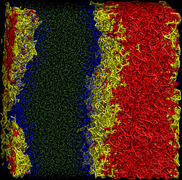
\includegraphics[width=1.4in]{A5B5_025} & 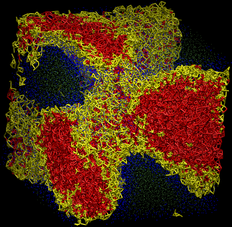
\includegraphics[width=1.4in]{A5B5_040} \\
		\rowcolor{black} \textcolor{white}{$w_{AB}=0.60$} & \textcolor{white}{$w_{AB}=0.65$} \\
		\rowcolor{black} 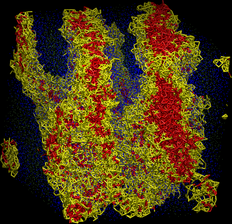
\includegraphics[width=1.4in]{A5B5_060} & 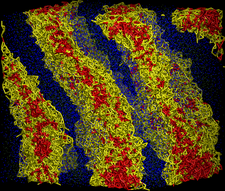
\includegraphics[width=1.4in]{A5B5_065} \\		
		\rowcolor{black} \textcolor{white}{$w_{AB}=0.75$} & \textcolor{white}{$w_{AB}=1.00$} \\
		\rowcolor{black} 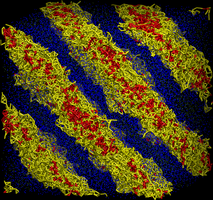
\includegraphics[width=1.4in]{A5B5_075} & 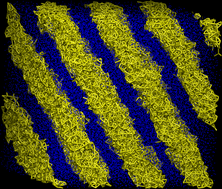
\includegraphics[width=1.4in]{A5B5_100} \\		
	\end{tabular}
	\caption{Selected structures formed in the simulations of the blend system using the \ce{A5B5} diblock copolymer.}
	\label{fig:Figure_2}
\end{figure}

\begin{figure}
	\centering
	\begin{tabular}{C{1.6in}@{}C{1.6in}}
		\includegraphics[width=1.6in]{figure_S26_025.pdf} & \includegraphics[width=1.6in]{figure_S26_040.pdf} \\
		\includegraphics[width=1.6in]{figure_S26_060.pdf} & \includegraphics[width=1.6in]{figure_S26_065.pdf} \\		\includegraphics[width=1.6in]{figure_S26_075.pdf} & \includegraphics[width=1.6in]{figure_S26_100.pdf} \\	
	\end{tabular}
	\caption{Structure-factor diagrams calculated for selected structures formed in the simulations of the blend system using the \ce{A5B5} diblock copolymer.}
	\label{fig:Figure_3}
\end{figure}

One can see in Fig.~\ref{fig:Figure_2} that the diblock copolymer, when present in small quantities, is adsorbed on the interface of the homopolymer phases.
As the copolymer concentration increases, the interface becomes saturated until it begins to form a curvature around $w_{AB}=0.25$.
A ``saturated surface'' is one which cannot afford further inclusion of copolymers without a change in its geometry.
However, as shown in Fig.~\ref{fig:Figure_3}, the structure factor in this condition still displays its maximum at the smallest value of $q$, indicating that a macrophase segregation still occurs \cite{Gavrilov_2013, Lemos_2020}.
When the copolymer mass fraction is $w_{AB}=0.40$, a main peak appears in $S(q)$, which is representative of the formation of mesostructures.
These incipient structures resemble connected tubes, but are poorly defined and strongly dependent on the mass fraction of copolymer in the mixture. 
At the mass fraction $w_{AB}=0.55$, the establishment of a lamellar mesostructure begins.
The signature of a lamellar structure is a secondary peak in $S(q)$ \cite{Gavrilov_2013, Lemos_2020}.
However, as one can observe in Fig.~\ref{fig:Figure_2}, the formed lamellae are initially defective, which is corroborated by the poor definition of the secondary peaks in the corresponding $S(q)$ diagram.
The lamellae are only fully established when $w_{AB}=0.75$ and, as the fraction of copolymers increases, the width of the lamellar domains decreases.
Therefore, in summary, the addition of diblock copolymers to immiscible homopolymers involves the following steps: \begin{enumerate*}[label=\roman*)] \item copolymer adsorption at the flat interface between homopolymer species, \item interface saturation with change in the interfacial geometry, \item formation of intermediate mesophases and, finally, \item formation of the same mesophase which the copolymer forms when pure.\end{enumerate*}

Increasing the amount of copolymers with homogeneous microstructure, such as \ce{A1B1A1B1A1B1A1B1A1B1}, leads to markedly different effect on the phase behavior of the blend.
This is shown in the three-dimensional pictures of Fig.~\ref{fig:Figure_4} and corresponding structure-factor diagrams in Fig.~\ref{fig:Figure_5}.
Unlike the diblock copolymer, which their block junctions lies at the interface with blocks merged into the respective homopolymer phases, alternate copolymers completely segregate to form a new phase.
When $w_{AB}=0.30$, the establishment of curved interfaces begins.
As more copolymer is added, the curvature undergoes modifications to accommodate the larger relative volume of the new phase.
It can be seen that homopolymers, whenever present, are almost entirely segregated, as the largest value of $S(q)$ placed at the lowest value of $q$ indicates.
Another interesting feature of Fig.~\ref{fig:Figure_5} is a bump in the $S(q)$ curve, which is formed at $q \approx 3.15$ and increases with the copolymer concentration.
This $q$ value indicates the occurrence of patterns in the order of the shortest distances between type-A beads in the copolymer chains, being representative of the segregated copolymeric phase.
Besides, two intermediate peaks can be clearly seen in the case of $w_{AB}=0.80$.
These peaks reflect the presence of homopolymer beads inserted in the copolymer matrix.

Based on the differences highlighted in this section, the effects of microstuctural dispersions are analyzed separately in the following sections for alternate copolymers (which do not form mesophasic structures when pures) and for diblock copolymers.

\begin{figure}
	\centering
	\begin{tabular}{C{1.6in}@{}C{1.6in}}
		\rowcolor{black} \textcolor{white}{$w_{AB}=0.20$} & \textcolor{white}{$w_{AB}=0.30$} \\
		\rowcolor{black} 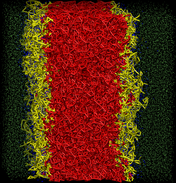
\includegraphics[width=1.4in]{alt1_020} & 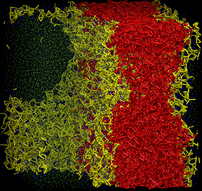
\includegraphics[width=1.4in]{alt1_030} \\
		\rowcolor{black} \textcolor{white}{$w_{AB}=0.60$} & \textcolor{white}{$w_{AB}=0.80$} \\
		\rowcolor{black} 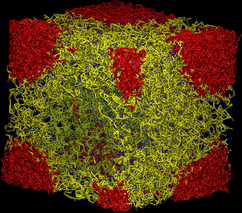
\includegraphics[width=1.4in]{alt1_060} & 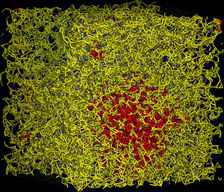
\includegraphics[width=1.4in]{alt1_080} \\		
		\rowcolor{black} \textcolor{white}{$w_{AB}=0.85$} & \textcolor{white}{$w_{AB}=1.00$} \\
		\rowcolor{black} 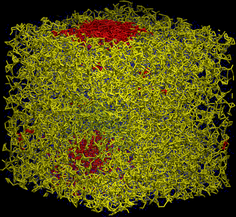
\includegraphics[width=1.4in]{alt1_085} & 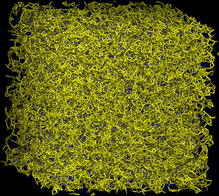
\includegraphics[width=1.4in]{alt1_100} \\		
	\end{tabular}
	\caption{Selected structures formed in the simulations of the blend system using the \ce{A1B1A1B1A1B1A1B1A1B1} copolymer system.}
	\label{fig:Figure_4}
\end{figure}

\begin{figure}
	\centering
	\begin{tabular}{C{1.6in}@{}C{1.6in}}
		\includegraphics[width=1.6in]{figure_S2_020.pdf} & \includegraphics[width=1.6in]{figure_S2_030.pdf} \\
		\includegraphics[width=1.6in]{figure_S2_060.pdf} & \includegraphics[width=1.6in]{figure_S2_080.pdf} \\		
		\includegraphics[width=1.6in]{figure_S2_085.pdf} & \includegraphics[width=1.6in]{figure_S2_100.pdf} \\		
	\end{tabular}
	\caption{Structure-factor diagrams calculated for selected structures formed in the simulations of the blend system using the \ce{A1B1A1B1A1B1A1B1A1B1} copolymer system.}
	\label{fig:Figure_5}
\end{figure}

\subsection{Alternate Copolymers}

In order to analyze the  influence of block lengths and their dispersions on the behaviour of the mixture, blends containing alternate copolymers with distinct microstructures were simulated, as shown in Table~\ref{table:copolymers}, with block lengths ranging from 1 to 3.
Among them, five copolymer species were considered, which are likely to be separated into 3 groups according to the average block length, as shown in Fig.~\ref{fig:Figure_6}. 

\begin{figure}
	\centering
	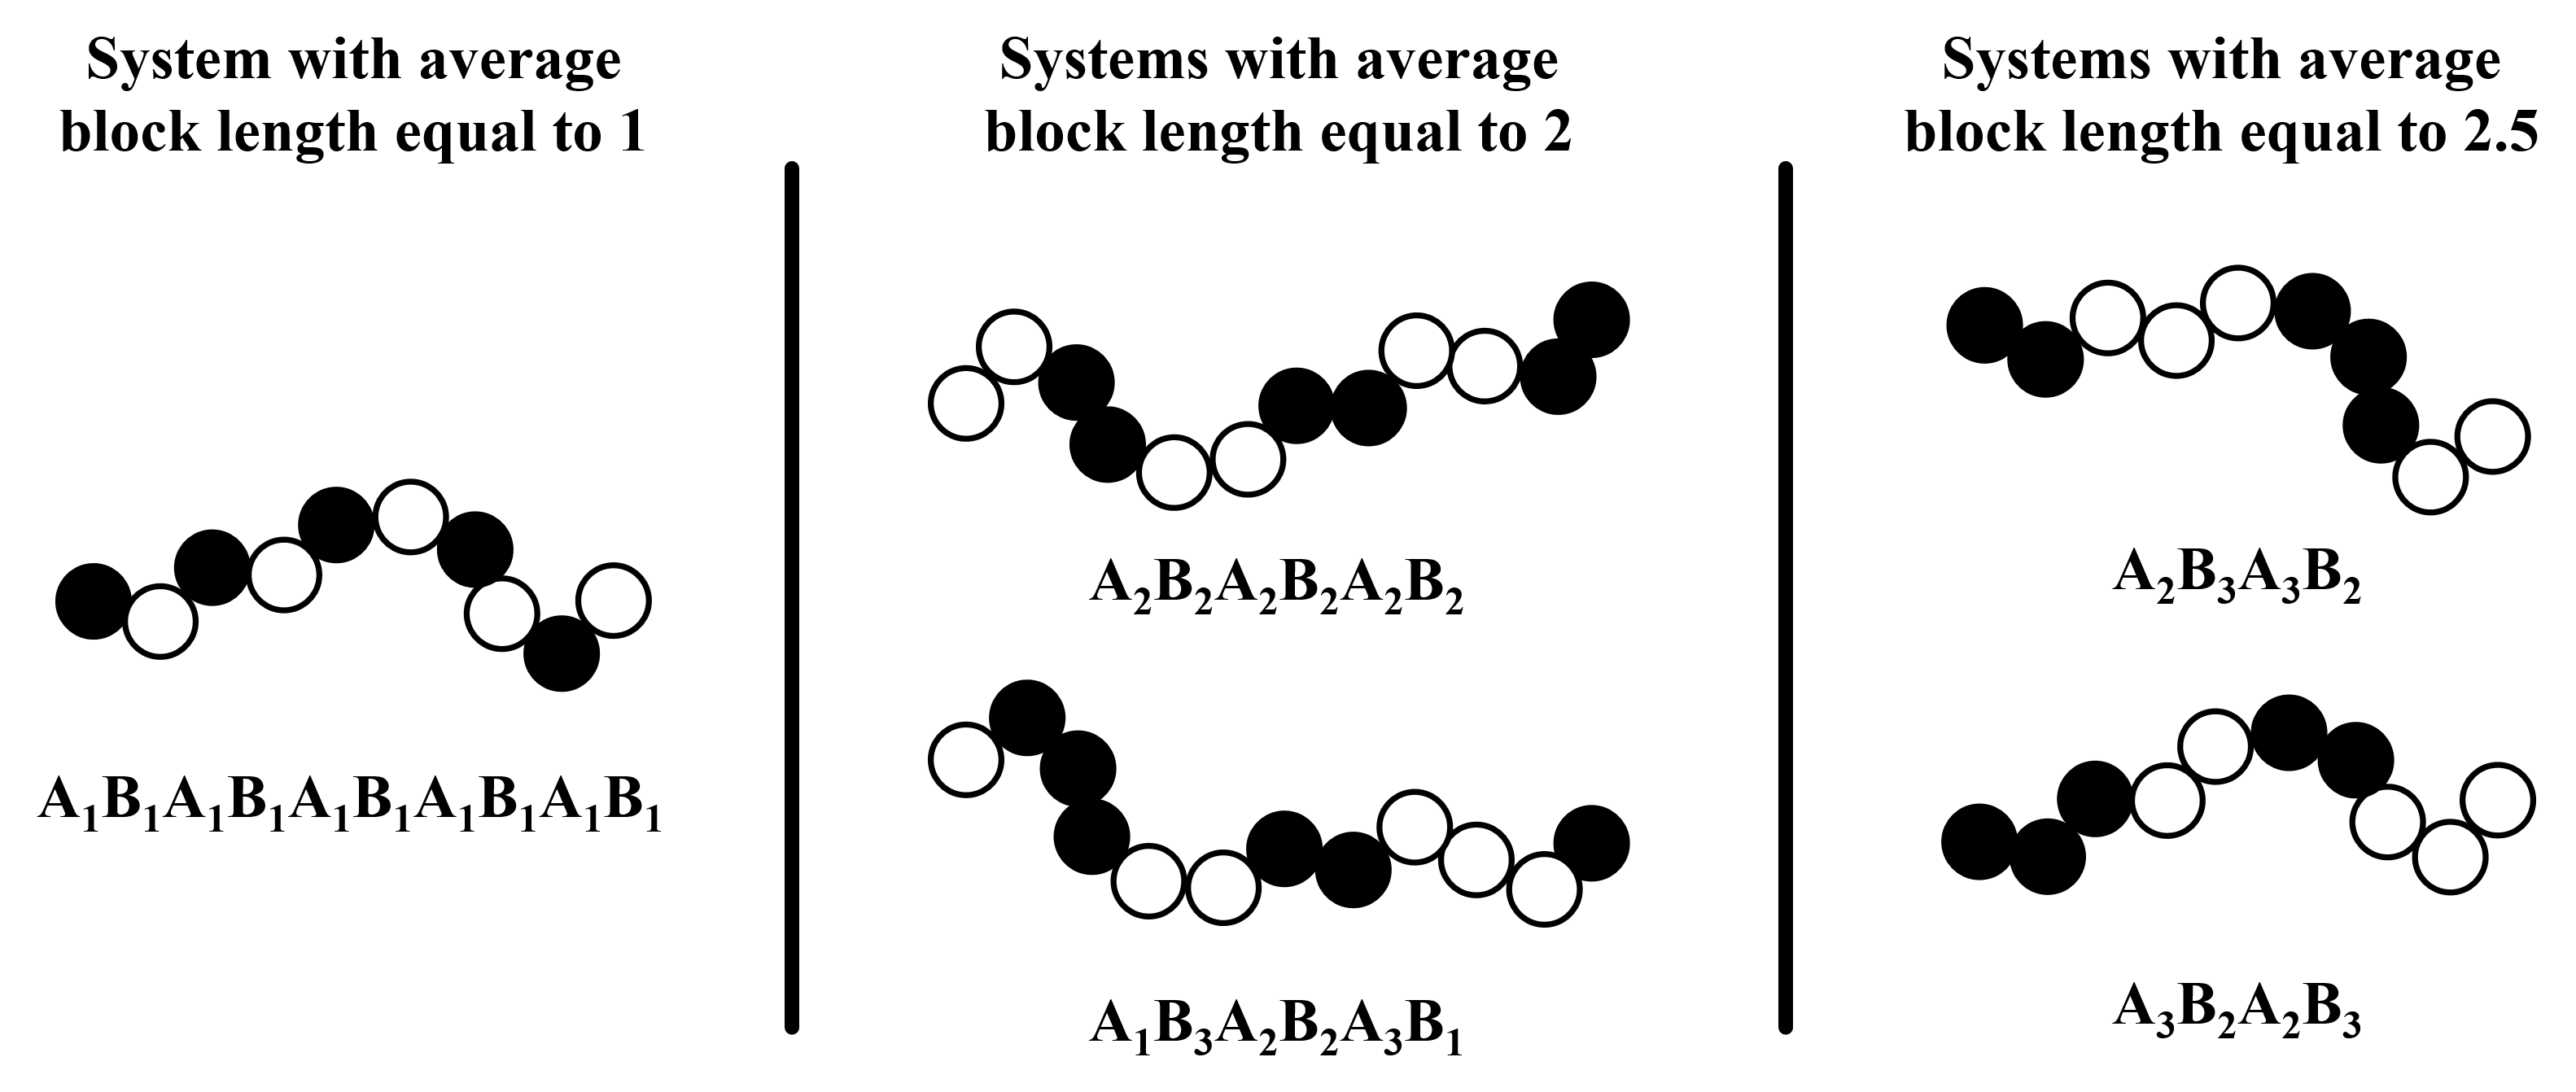
\includegraphics[width=3.2in]{figure6.png}
	\caption{Alternate copolymer systems with fraction of type-A component $f_A=0.50$  separated according to the average length of the segments.}
	\label{fig:Figure_6}
\end{figure}

Alternate copolymers form a disordered isotropic phase, but with nanodomains that are rich in each component.
Such nanodomains become larger as the blocks that constitute the copolymer chains increase in size.
Such result is illustrated in Fig.~\ref{fig:Figure_7} by analyzing the $q$ values where $S(q)$ attains the supreme value, $q_\mathrm{sup}$.
As already mentioned, the characteristic sizes are inversely proportional to the value of $q_\mathrm{sup}$.
It is noteworthy on Fig.~\ref{fig:Figure_7} that the points of $q_\mathrm{sup}$ in the lowest value of q sampled $q_\mathrm{sup} = 0.251$ indicate the systems that present phases consisting of homopolymers.

\begin{figure}
	\centering
	\includegraphics[width=3.2in]{figure7}
	\caption{Supreme $q$ values found in structure-factor diagrams calculated for simulations using alternate copolymers with fraction of type-A component $f_A=0.50$ .}
	\label{fig:Figure_7}
\end{figure}

The difference in size of the generated nanodomains also impacts the mixing behavior in respect to the homopolymer chains present.
It is noticed that the segregated nanodomains become larger also due to their capacity of incorporating the homopolymer chains.
This can be seen in the 3D structures and corresponding structure-factor diagrams shown in Fig.~\ref{fig:Figure_8}, simulation results obtained with $w_{AB}=0.95$ for the copolymers which form the smallest (\ce{A1B1A1B1A1B1A1B1A1B1}) and the largest (\ce{A3B2A2B3}) nanodomains are analyzed.

\begin{figure}
	\centering
	\begin{tabular}{C{1.6in}@{}C{1.6in}}
		\rowcolor{black} \textcolor{white}{ \ce{A1B1A1B1A1B1A1B1A1B1}} & \textcolor{white}{ \ce{A3B2A2B3}} \\
		\rowcolor{black} 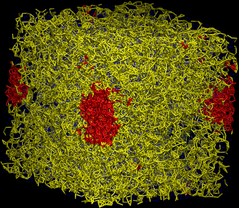
\includegraphics[width=1.4in]{alt1_095} & 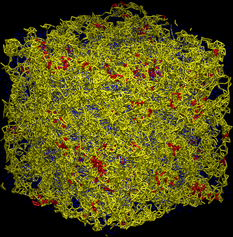
\includegraphics[width=1.4in]{A3B2A2B3_095} \\
		\multicolumn{2}{c}{\includegraphics[width=3.0in]{figure8b}} \\
	\end{tabular}
	\caption{(top) Structures formed in the simulations using the copolymeric systems \ce{A1B1A1B1A1B1A1B1A1B1} and \ce{A3B2A2B3} with $w_{AB}=0.95$ and (bottom) respective structure-factor diagrams.}
	\label{fig:Figure_8}
\end{figure}

Fig.~\ref{fig:Figure_8} reveals that copolymer \ce{A3B2A2B3} completely incorporates the homopolymer chains into its phase matrix, so that homopolymeric phases are not formed.
Similar results can also be seen in Fig.~\ref{fig:Figure_7}, where it is possible to see that larger copolymer domains are formed for larger copolymer blocks, with more efficient incorporation of homopolymer chains in the copolymer nanodomains.
Systems for which $q_\mathrm{sup} \neq 0.251$ are those without homopolymer phases.
The copolymers \ce{A1B3A2B2A3B1} and \ce{A2B2A2B2A2B2} differ only in terms of the dispersion of block lengths, as both systems present the same fraction of type-A component, chain length, and average block length.
It can also be seen in Fig.~\ref{fig:Figure_7} that the nanodomains of the \ce{A1B3A2B2A3B1}-containing system are larger than those of the \ce{A2B2A2B2A2B2}-containing one.
This result indicates that the increase of the microstructural inhomogeneity, in this case the dispersion in the block lengths, causes the system to extend its degree of segregation.
A possible explanation is that the existence of different block lengths assists the relief of torsions and stretches, as compared to the case in which all blocks have the same length, in analogy to what occurs in the self-assembly of diblock copolymers \cite{Matsen_2006, Lemos_2020}.
In diblock copolymers, the variety in chain lengths makes the self-assembly process more effective because the smaller blocks fill the domains closest to the interfacial region while the larger blocks fill the interior of the mesophases, in order to avoid unfavorable torsions and stretches \cite{Matsen_2006, Lemos_2020}.
The copolymer chains \ce{A2B3A3B2} and \ce{A3B2A2B3} have, in addition to the same length and type-A component fraction, exactly the same block-length distribution.
The difference between them is that the largest blocks occupy the ends of the \ce{A3B2A2B3} chains, thus being subjected to only one block junction, while in the case of \ce{A2B3A3B2} the largest blocks are in the middle of the chain, thus having connections to two other blocks each.
It can be seen in Fig.~\ref{fig:Figure_9} that $S(q)$ captures sensitively and satisfactorily well the differences in nanodomain sizes, although visually this difference may be almost indiscernible.
Therefore, it appears that the number of block junctions to which the largest blocks are subjected appreciably constrains their freedom to segregate from incompatible components. Apparently, this effect has never been discussed in the literature.

\begin{figure}
	\centering
	\begin{tabular}{C{1.6in}@{}C{1.6in}}
		\rowcolor{black} \textcolor{white}{ \ce{A2B3A3B2}} & \textcolor{white}{ \ce{A3B2A2B3}} \\
		\rowcolor{black} 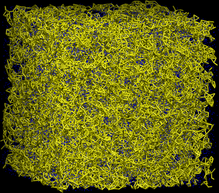
\includegraphics[width=1.4in]{A2B3A3B2_100} & 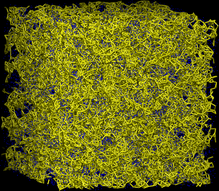
\includegraphics[width=1.4in]{A3B2A2B3_100} \\
		\multicolumn{2}{c}{\includegraphics[width=3.0in]{figure9b}} \\
	\end{tabular}
	\caption{(top) Structures formed in the simulations using the copolymeric systems \ce{A2B3A3B2} and \ce{A3B2A2B3} with $w_{AB}=1.00$ and (bottom) respective structure-factor diagrams.}
	\label{fig:Figure_9}
\end{figure}

Systems with copolymers \ce{A1B3A2B2A3} and \ce{A2B2A2B2A2}, for which $\bar{f}_A \neq 0.50$, behave similarly to the previously described systems.
For these cases, images of formed 3D structures and corresponding structure factors can be found in the Support Information.

\subsection{Diblock Copolymers: Effects of Dispersion in the Chain Length Distribution}
\label{sec:CLD effects}

In this section, the influence of the chain length distribution (CLD) of compatibilizing diblock copolymers on the blend properties is investigated.
This is done by comparing simulations using either a non-dispersed \ce{A5B5} copolymer or a Flory-distributed copolymeric mixture for which $\bar{f}_A = 0.50$ and $( \overline{DP} )_{AB} = 10$.
Some selected 3D structures obtained in these simulations are shown in Fig.~\ref{fig:Figure_10}, with their respective structure-factor diagrams.

\begin{figure}
	\centering
	\begin{tabular}{C{1.6in}@{}C{1.6in}}
		\rowcolor{black}  \textcolor{white}{\ce{A5B5}} & \textcolor{white}{Flory-type} \\
		\rowcolor{black} \multicolumn{2}{c}{\textcolor{white}{$w_{AB}=0.30$}} \\
		\rowcolor{black} 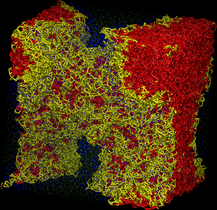
\includegraphics[width=1.4in]{A5B5_030} & 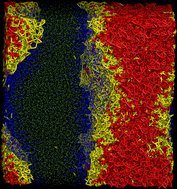
\includegraphics[width=1.4in]{A5B5_Flory_030} \\
		\rowcolor{black} \multicolumn{2}{c}{\textcolor{white}{$w_{AB}=0.50$}} \\
		\rowcolor{black} 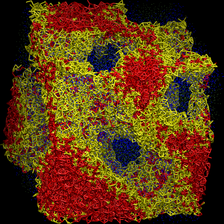
\includegraphics[width=1.4in]{A5B5_050} & 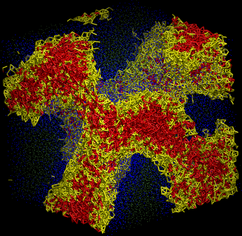
\includegraphics[width=1.4in]{A5B5_Flory_050} \\
    	\rowcolor{black} \multicolumn{2}{c}{\textcolor{white}{$w_{AB}=0.55$}} \\\rowcolor{black} 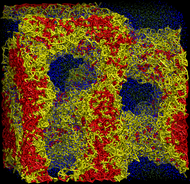
\includegraphics[width=1.4in]{A5B5_055} & 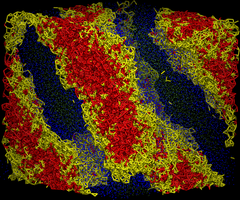
\includegraphics[width=1.4in]{A5B5_Flory_055} \\
		\rowcolor{black} \multicolumn{2}{c}{\textcolor{white}{$w_{AB}=0.80$}} \\\rowcolor{black} 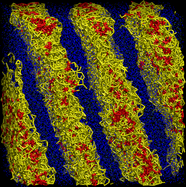
\includegraphics[width=1.4in]{A5B5_080} & 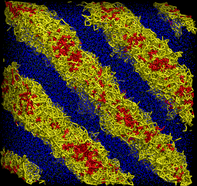
\includegraphics[width=1.4in]{A5B5_Flory_080} \\
		%\multicolumn{2}{c}{\includegraphics[width=3.0in]{figure10b}} \\
		\includegraphics[width=1.6in]{figure10_030.pdf} & \includegraphics[width=1.6in]{figure10_050.pdf} \\
		\includegraphics[width=1.6in]{figure10_055.pdf} & \includegraphics[width=1.6in]{figure10_080.pdf}
	\end{tabular}
	\caption{(top) Structures formed in some selected simulations using either the \ce{A5B5} copolymer or a CLD distributed copolymer mixture and (bottom) respective structure-factor diagrams.}
	\label{fig:Figure_10}
\end{figure}

It can be seen in Fig.~\ref{fig:Figure_10}, both in the 3D structures and in the location of peaks in $S(q)$, that the domains generated in the dispersed case are significantly larger than those generated in the non-dispersed case.
Increasing the amount of length-distributed copolymers in the blend resulted in the structural changes that were similar to the onse observed by adding non-dispersed copolymers.
However, as summarized in Table~\ref{table:steps}, transitions in the dispersed case occurred at larger values of copolymer mass fraction $w_{AB}$ than their equivalent transitions in the non-dispersed case.

\begin{table*}
	\centering
	\caption{Steps of the process of increasing the amount of copolymers in simulations of blends using either a non-dispersed or a dispersed copolymer samples.}
	\begin{tabular*}{\textwidth}{@{\extracolsep{\fill}}lcc}
		\hline\hline
\multirow{2}{*}{Phenomenon} & $w_{AB}$ & $w_{AB}$ \\
& (\ce{A5B5}) & (Flory-type) \\
\hline
Copolymer adsorption at the flat interface of homopolymers & 0.05-0.20 & 0.05-0.25 \\
Flat interface saturation & 0.25 & 0.30 \\
Curved Interface & 0.30-0.35 & 0.35-0.45 \\
Onset of mesophase segregation & 0.40-0.50 & 0.50 \\
Establishment of defective lamellae & 0.55-0.70 & 0.55-0.75 \\
Fully-formed lamellae & 0.75-1.00 & 0.80-1.00 \\
		\hline\hline
		\label{table:steps}
	\end{tabular*}
\end{table*}

Fig.~\ref{fig:Figure_11} shows $q_\mathrm{sup}$ as a function of the copolymer mass fraction.
Lower values of $q_\mathrm{sup}$, which denote larger characteristic domain sizes, are evident for the dispersed case.

\begin{figure}
	\centering
	\includegraphics[width=3.2in]{figure11}
	\caption{Supreme $q$ values found in structure-factor diagrams calculated from simulations using \ce{A5B5} and CLD distributed copolymers.}
	\label{fig:Figure_11}
\end{figure}

It seems that the existence of chain segments with different lengths causes a hierarchy in the process of filling of the segregated domains: block junctions always lie at the interface, but blocks of different lengths are more efficient during the segregation process because smaller blocks preferably occupy the regions that are closer to the interface and the larger blocks fill the center of the mesophasic structures.
This reduces, in this process of filling the core of the mesostructures, the occurrence of unfavorable torsions and stretches, corroborating previous results \cite{Matsen_2006, Gavrilov_2013, Lemos_2020}. 

\subsection{Diblock Copolymers: Effects of Dispersion in the Chemical Composition Distribution}
\label{sec:CCD effects}

In order to analyze the effect of dispersion of the CCD of the added copolymers, simulations involving copolymer mixtures that have bidisperse CCD's with different variances were performed.
Besides the non-dispersed case \ce{A5B5}, equimolar mixtures of diblock copolymers were considered, expressed as $\ce{A_nB_m + A_mB_n}$, with $n+m=10$, thus resulting in $\bar{f}_A = 0.50$ in all cases.
%\ce{A1B9 + A9B1}, \ce{A2B8 + A8B2}, \ce{A3B7 + A7B3} and \ce{A4B6 + A6B4}, and the \ce{A5B5} non-dispersed case.
Table~\ref{table:dynamics} summarizes the equilibrium mesophases observed in these simulations in the whole range of analyzed copolymer mass fractions.

\begin{sidewaystable}
	\centering
	\caption{Mesophase behavior resulting from varying the amount of copolymers, with different levels of dispersion in their chemical composition distributions, in a blend with non-compatible homopolymers.}
	\begin{tabular*}{\textwidth}{@{\extracolsep{\fill}}cccccc}
		\hline\hline
$w_{AB}$ & \ce{A1B9 + A9B1} & \ce{A2B8 + A8B2} & \ce{A3B7 + A7B3} & \ce{A4B6 + A6B4} & \ce{A5B5} \\
\hline
0.05 & \biphasic & \biphasic & \biphasic & \biphasic & \biphasic \\
0.10 & \biphasic & \biphasic & \biphasic & \biphasic & \biphasic \\
0.15 & \biphasic & \biphasic & \biphasic & \biphasic & \biphasic \\
0.20 & \biphasic & \biphasic & \biphasic & \biphasic & \biphasic \\
0.25 & \biphasic & \biphasic & \saturatedflatinterface & \saturatedflatinterface & \saturatedflatinterface \\
0.30 & \biphasic & \saturatedflatinterface & \curvedinterface & \curvedinterface & \curvedinterface \\
0.35 & \biphasic & \curvedinterface & \curvedinterface & \curvedinterface & \curvedinterface \\
0.40 & \biphasic & \curvedinterface & \mesophasic & \mesophasic & \mesophasic \\
0.45 & \biphasic & \curvedinterface & \mesophasic & \mesophasic & \mesophasic \\
0.50 & \biphasic & \mesophasic & \mesophasic & \mesophasic & \mesophasic \\
0.55 & \biphasic & \mesophasic & \mesophasic & \mesophasic & \defectivelamellae \\
0.60 & \biphasic & \mesophasic & \defectivelamellae & \defectivelamellae & \defectivelamellae \\
0.65 & \biphasic & \defectivelamellae & \defectivelamellae & \defectivelamellae & \defectivelamellae \\
0.70 & \biphasic & \defectivelamellae & \defectivelamellae & \defectivelamellae & \defectivelamellae \\
0.75 & \biphasic & \defectivelamellae & \lamellae & \lamellae & \lamellae \\
0.80 & \biphasic & \defectivelamellae & \lamellae & \lamellae & \lamellae \\
0.85 & \biphasic & \lamellae & \lamellae & \lamellae & \lamellae \\
0.90 & \biphasic & \lamellae & \lamellae & \lamellae & \lamellae \\
0.95 & \biphasic & \lamellae & \lamellae & \lamellae & \lamellae \\
1.00 & \biphasic & \lamellae & \lamellae & \lamellae & \lamellae \\
		\hline\hline
\label{table:dynamics}
\end{tabular*}
\end{sidewaystable}

The case \ce{A1B9 + A9B1}, as one can observe in Fig.~\ref{fig:Figure_12}, forms two immiscible phases regardless of the amount of copolymers in the system.
This behavior differs from the one observed with the diblock copolymer \ce{A5B5}.
The copolymers are incorporated into the phases with which they are mostly compatible, i.e. the \ce{A9B1} chains occupy the phase formed by the type-A homopolymer while the \ce{A1B9} chains occupy the phase formed by the type-B homopolymer.
The largest block of each chain is able to carry the single opposite-type bead to the core of a phase, meaning that block junctions do not necessarily lie at the interface.
This is corroborated by the $S(q)$ diagram in Fig.~\ref{fig:Figure_12}.
One can note that the biphasic structure is not affected by an increase in the copolymer content, but the phase purity decreases due to contamination by the single beads of opposite type, since $S(q)$ has higher values for the entire $q$ range.

\begin{figure}
	\centering
	\begin{tabular}{C{1.6in}@{}C{1.6in}}
		\rowcolor{black} \textcolor{white}{$w_{AB}=0.25$} & \textcolor{white}{$w_{AB}=0.50$} \\
		\rowcolor{black} 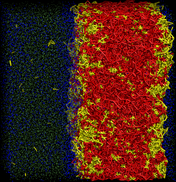
\includegraphics[width=1.4in]{A1B9_A9B1_025} & 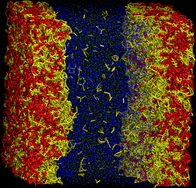
\includegraphics[width=1.4in]{A1B9_A9B1_050} \\
		\rowcolor{black} \textcolor{white}{$w_{AB}=0.75$} & \textcolor{white}{ $w_{AB}=1.00$} \\
		\rowcolor{black} 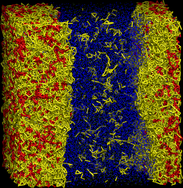
\includegraphics[width=1.4in]{A1B9_A9B1_075} & \includegraphics[width=1.4in]{A1B9_A9B1_100} \\
		\multicolumn{2}{c}{\includegraphics[width=3.0in]{figure12b}} \\
	\end{tabular}
	\caption{(top) Structures formed in some selected simulations using the \ce{A1B9 + A9B1} copolymer system and (bottom) respective structure-factor diagrams.}
	\label{fig:Figure_12}
\end{figure}

The other cases with bidispersed CCD's presented the same structural changes already discussed for the \ce{A5B5} case due to increase of the copolymer content.
Although the transition steps are the same, the copolymer mass fractions in which they occur, as well as the characteristic sizes of the involved segregated domains, depend on the degree of dispersion in the CCD.
These results are similar to the effect of CLD observed in the previous section.
In Fig.~\ref{fig:Figure_13}, the final configurations and structure-factor diagrams for the analyzed systems are observed when $w_{AB}=0.25$.
For this condition, the copolymer mixture \ce{A2B8 + A8B2} results in a flat rather than a saturated interface.
For the other three cases, the interface is saturated, presenting layered copolymeric chains.
It is also possible to notice that in the case of \ce{A2B8 + A8B2}, the homopolymeric phases contain more impurities, meaning that some copolymer chains are fully inserted into the domain corresponding to their major components.
This may explain the insaturation of the interface, since fewer strings occupy the interface as compared to cases of copolymers with less dispersed CCD's.

\begin{figure}
	\centering
	\begin{tabular}{C{1.6in}@{}C{1.6in}}
		\rowcolor{black} \textcolor{white}{\ce{A2B8 + A8B2}} & \textcolor{white}{\ce{A3B7 + A7B3}} \\
		\rowcolor{black} \includegraphics[width=1.4in]{A2B8_A8B2_025} & \includegraphics[width=1.4in]{A3B7_A7B3_025} \\
		\rowcolor{black} \textcolor{white}{\ce{A4B6 + A6B4}} & \textcolor{white}{ \ce{A5B5}} \\
		\rowcolor{black} \includegraphics[width=1.4in]{A4B6_A6B4_025} & \includegraphics[width=1.4in]{A5B5_025} \\
        \includegraphics[width=1.6in]{figure13_A2B8_A8B2_025.pdf} & \includegraphics[width=1.6in]{figure13_A3B7_A7B3_025.pdf} \\
		\includegraphics[width=1.6in]{figure13_A4B6_A6B4_025.pdf} & \includegraphics[width=1.6in]{figure13_A5B5_025.pdf}
	\end{tabular}
	\caption{(top) Structures formed in the diblock copolymer that exhibit different CCD's: \ce{A2B8 + A8B2}, \ce{A3B7 + A7B3}, \ce{A4B6 + A6B4}, and \ce{A5B5} with $w_{AB}=0.25$ and (bottom) respective structure-factor diagrams.}
	\label{fig:Figure_13}
\end{figure}

In Fig.~\ref{fig:Figure_14}, the final structures and respective structure-factor diagrams for the same systems when $w_{AB}=0.75$ are shown.
The behavior is similar to the one previously observed for $w_{AB}=0.25$, so that while systems where copolymers with a smaller CCD dispersion are added already present well-defined lamellae, the \ce{A2B8 + A8B2} case shows, as in lower concentrations of copolymers,  defective lamellae.
This shows a similar behavior to that seen in the previous section, of the case in the study of the effect of CLD, in which larger amounts of dispersed copolymers were necessary to cause changes in the behavior of the mixture, in comparison to the amount of non-dispersed copolymers.

One can also visualize in Fig.~\ref{fig:Figure_14} the effect of CCD dispersion on the domain sizes, with the least dispersed copolymer microstructures being the ones that generate the narrowest lamellae.

\begin{figure}
	\centering
	\begin{tabular}{C{1.6in}@{}C{1.6in}}
		\rowcolor{black} \textcolor{white}{\ce{A2B8 + A8B2}} & \textcolor{white}{\ce{A3B7 + A7B3}} \\
		\rowcolor{black} \includegraphics[width=1.4in]{A2B8_A8B2_075} & \includegraphics[width=1.4in]{A3B7_A7B3_075} \\
		\rowcolor{black} \textcolor{white}{\ce{A4B6 + A6B4}} & \textcolor{white}{ \ce{A5B5}} \\
		\rowcolor{black} \includegraphics[width=1.4in]{A4B6_A6B4_075} & \includegraphics[width=1.4in]{A5B5_075} \\
        \includegraphics[width=1.6in]{figure14_A2B8_A8B2_075.pdf} & \includegraphics[width=1.6in]{figure14_A3B7_A7B3_075.pdf} \\
		\includegraphics[width=1.6in]{figure14_A4B6_A6B4_075.pdf} & \includegraphics[width=1.6in]{figure14_A5B5_075.pdf}	\end{tabular}
	\caption{(top) Structures formed in the diblock copolymers that exhibit different CCDs: \ce{A2B8 + A8B2}, \ce{A3B7 + A7B3}, \ce{A4B6 + A6B4} and \ce{A5B5} with $w_{AB}=0.75$ and (bottom) respective structure-factor diagrams.}
	\label{fig:Figure_14}
\end{figure}

In Fig.~\ref{fig:Figure_15}, one can observe the final structures and structure-factor diagrams for pure copolymer simulations ($w_{AB}=1.00$), in which it is possible to notice, by means of the lamellar thicknesses, that the greater the dispersions in the CCD, the larger the domains formed.
This result is also present in Fig.~\ref{fig:Figure_16}, which shows  the $q$ values where $S(q)$ attains the supreme values, and in which it is possible to see how the dispersion of the CCD result in smaller values of $q$, thus denoting larger sizes of characteristic domains.

\begin{figure}
	\centering
	\begin{tabular}{C{1.6in}@{}C{1.6in}}
		\rowcolor{black} \textcolor{white}{\ce{A2B8 + A8B2}} & \textcolor{white}{\ce{A3B7 + A7B3}} \\
		\rowcolor{black} \includegraphics[width=1.4in]{A2B8_A8B2_100} & \includegraphics[width=1.4in]{A3B7_A7B3_100} \\
		\rowcolor{black} \textcolor{white}{\ce{A4B6 + A6B4}} & \textcolor{white}{ \ce{A5B5}} \\
		\rowcolor{black} \includegraphics[width=1.4in]{A4B6_A6B4_100} & \includegraphics[width=1.4in]{A5B5_100} \\
        \includegraphics[width=1.6in]{figure15_A2B8_A8B2_100.pdf} & \includegraphics[width=1.6in]{figure15_A3B7_A7B3_100.pdf} \\
		\includegraphics[width=1.6in]{figure15_A4B6_A6B4_100.pdf} & \includegraphics[width=1.6in]{figure15_A5B5_100.pdf}	\end{tabular}
	\caption{(top) Structures formed with diblock copolymers that exhibit different CCDs: \ce{A2B8 + A8B2}, \ce{A3B7 + A7B3}, \ce{A4B6 + A6B4} and \ce{A5B5} with $w_{AB}=1.00$ condition and (bottom) respective structure-factor diagrams.}
	\label{fig:Figure_15}
\end{figure}

\begin{figure}
	\centering
	\includegraphics[width=3.2in]{figure16}
	\caption{Supreme $q$ values found in the structure-factor diagrams calculated for simulations using copolymers with different degrees of dispersion in their chemical composition distributions.}
	\label{fig:Figure_16}
\end{figure}

It can be noted that both the CCD dispersion control and the copolymer concentration can be used as variables to adjust the characteristic sizes of formed mesophases.
Analyzing Table~\ref{table:dynamics} and Fig.~\ref{fig:Figure_16}, it can be seen that the broader lamellae were formed in the simulation using copolymer \ce{A3B7 + A7B3} at a mass fraction of $w_{AB}=0.75$ (or \ce{A2B8 + A8B2} at $w_{AB}=0.85$), where $q_\mathrm{sup}=0.711$.
On the other hand, pure \ce{A5B5} non-dispersed copolymer formed the narrowest lamellae, with $q_\mathrm{sup}=0.940$.
By calculating the interlamellar distances $L$, by Eq.~\eqref{eq:characteristic size}, the difference between the thicknesses of the lamellar domains was 2.16, meaning that the lamellae can dilate up to 30\% by adding homopolymers and properly controlling the dispersion level of the CCD of the copolymer systems.

\subsection{The \ce{A3B7} Diblock Copolymer Case}

The justification for the use of the \ce{A3B7} copolymeric system lies in the fact that such copolymer, when pure, forms hexagonally packed cylinders, which finds applications that are different from the ones based on lamellar mesostructures. Besides, it is interesting to observe how the mixture develops with copolymers of different fractions of type-A component.
Fig.~\ref{fig:Figure_17} shows the structures at the end of each simulation and Fig.~\ref{fig:Figure_18} shows the respective structure-factor diagrams. 

\begin{figure}
	\centering
	\begin{tabular}{C{1.6in}@{}C{1.6in}}
		\rowcolor{black} \textcolor{white}{$w_{AB}=0.25$} & \textcolor{white}{$w_{AB}=0.40$} \\
		\rowcolor{black} \includegraphics[width=1.4in]{A3B7_025} & \includegraphics[width=1.4in]{A3B7_040} \\
		\rowcolor{black} \textcolor{white}{$w_{AB}=0.75$} & \textcolor{white}{$w_{AB}=0.85$} \\
		\rowcolor{black} \includegraphics[width=1.4in]{A3B7_075} & \includegraphics[width=1.4in]{A3B7_085} \\		
		\rowcolor{black} \textcolor{white}{$w_{AB}=0.90$} & \textcolor{white}{$w_{AB}=1.00$} \\
		\rowcolor{black} \includegraphics[width=1.4in]{A3B7_090} & \includegraphics[width=1.4in]{A3B7_100} \\		
	\end{tabular}
	\caption{Selected structures formed in the simulations performed with the \ce{A3B7} copolymer system.}
	\label{fig:Figure_17}
\end{figure}


\begin{figure}
	\centering
	\begin{tabular}{C{1.6in}@{}C{1.6in}}
		\includegraphics[width=1.6in]{figure_S20_025.pdf} & \includegraphics[width=1.6in]{figure_S20_040.pdf} \\
		\includegraphics[width=1.6in]{figure_S20_075.pdf} & \includegraphics[width=1.6in]{figure_S20_085.pdf} \\		\includegraphics[width=1.6in]{figure_S20_090.pdf} & \includegraphics[width=1.6in]{figure_S20_100.pdf} \\	
	\end{tabular}
	\caption{Structure-factor diagrams calculated for selected structures formed in the simulations performed with the \ce{A3B7} copolymer system.}
	\label{fig:Figure_18}
\end{figure}

%\begin{figure*}
	%\centering
	%\includegraphics[width=6.5in]{figure18}
	%\caption{Structure-factor diagrams calculated for final structures formed in the simulations of the blend system using the \ce{A3B7} copolymer system.}
	%\label{fig:Figure_18}
%\end{figure*}

It can be seen that the behavior differs slightly from the one observed for the diblock copolymer systems studied in the previous sections.
For low values of $w_{AB}$, the copolymer is adsorbed at the flat interface between phases.
At intermediate values, due to the change in fraction of type-A component, the interface is no longer flat and appears as a large spherical macrophasic domain.
Higher amounts of copolymer chains cause breakage of this spherical drop to form micellar domains.
The increase in the copolymer mass fraction causes the micellar concentration to increase, so that the copolymer presents a surfactant action.
When $w_{AB}=0.75$, the micellar domains begin to stretch, forming worm-like micelles.
The elongation is accentuated up to the point where the mass fraction of the copolymer is $w_{AB}=0.85$. At $w_{AB}=0.90$, coalescence of these elongated micelles occurs, giving birth to cylinders, albeit poorly formed.
At $w_{AB}=0.95$, the cylinders are fully established.
Therefore, the equimolar mixture of incompatible homopolymers and copolymer chains with $f_A=0.30$ is capable of forming spherical and worm-like micelles, with the copolymer fraction being able to control the micellar domain sizes over a wide range of compositions.

\section{Conclusions}
\label{sec:conclusions}

In the present paper, several aspects were investigated regarding how the microstructure of a copolymer affects the properties of a blend in which it participates as the compatibilizing agent between two incompatible homopolymers.
Alternate copolymers exhibit a simple behavior, forming a separate phase located between the immiscible homopolymers.

The effect of increasing the mass fraction of the alternate copolymers proved to be simpler than that of doing it for diblock, forming a copolymer phase that is arranged between the homopolymer phases.

Depending on the length of the copolymer blocks, nanodomains rich in each of the components can be formed in the middle of the copolymer phase and homopolymer chains can get allocated inside these nanodomains.

In addition to the expected fact that larger nanodomains are formed with larger block sizes and that, consequently, this can lead to higher insertion of homopolymer chains into the copolymer matrix, the results also showed that dispersions in the block lengths can also have the same effect.

Another factor that can change the size of the formed domains is the amount of junctions to which the blocks are subjected. Chains with larger terminal blocks resulted in larger domains, when compared to chains with the largest blocks placed inside.

For diblock copolymers with fraction of type-A component $f_A=0.50$, the increase of the mass fraction caused the following sequence of facts: \begin{enumerate*}[label=\roman*)] \item adsorption of copolymer at interface of non-compatible phases, \item interface saturation with interfacial geometry change, \item formation of intermediate mesophases, and \item formation of the mesophase that the pure copolymer forms (lamellae).\end{enumerate*}

Dispersions in CLD and CCD caused the formed mesophasic domains to increase. In addition, larger amounts of copolymers are required to cause changes in the mixing behavior, when compared to added amounts of non-dispersed copolymers.

Diblock copolymers with composition $f_A=0.30$ played a surfactant function in simulations that proved possible to regulate micelle size through appropriate control of the amount of copolymer added to the system.
Therefore, it can be seen that the microstructural properties of the copolymer decisively impact the morphological characteristics of mesophases generated in the mixing of non-compatible homopolymers, as well as the size and purity of formed domains.
This means that microstructure control methods, both from polymer reaction engineering and polymer purification techniques, can be important for the design and performance of blends formed by non-compatible homopolymers and copolymers. 

\begin{acknowledgement}

The authors thank CAPES (Coordena\c{c}\~ao de Aperfei\c{c}oamento de Pessoal de N\'ivel Superior), CNPq (Conselho Nacional de Desenvolvimento Cient\'ifico e Tecnol\'ogico), and FAPERJ (Funda\c{c}\~ao Carlos Chagas Filho de Apoio a Pesquisa do Estado do Rio de Janeiro) for financial support and scholarships.

\end{acknowledgement}

\bibliography{references}

\begin{tocentry}
	\includegraphics[width=\linewidth]{ToCfigure}
	Our DPD simulations show that the copolymer microstructural properties have a decisive impact on the interaction and mesophases generated in the mixing process with non-compatible homopolymers.
	So that the microstructure control methods, derived from polymer reaction engineering or from polymer purification, are important for to design and performance of these blends.
\end{tocentry}

\end{document}